\documentclass[11pt,letterpaper]{article}
\usepackage{naaclhlt2016}
\usepackage{times}
\usepackage{latexsym}

% More packages
\usepackage{amsmath}
\usepackage{amssymb}
\usepackage{graphicx}
\usepackage{hyperref}
\usepackage{xspace}

% Some helpful macros
%% Abbreviations
\newcommand{\encdec}{\textsc{EncDec}\xspace}
\newcommand{\attn}{\textsc{Attn}\xspace}
\newcommand{\attncopy}{\textsc{AttnCopy}\xspace}
\newcommand{\atis}{\textsc{ATIS}\xspace}
\newcommand{\regex}{\textsc{Regex}\xspace}
\newcommand{\geo}{\textsc{Geo}\xspace}

%% Mathematical Notation
\newcommand{\vocabin}{\mathcal{V}^{\text{(in)}}}
\newcommand{\phiin}{\phi^{\text{(in)}}}
\newcommand{\vocabout}{\mathcal{V}^{\text{(out)}}}
\newcommand{\phiout}{\phi^{\text{(out)}}}

\naaclfinalcopy % Uncomment this line for the final submission
\def\naaclpaperid{***} %  Enter the naacl Paper ID here

% To expand the titlebox for more authors, uncomment
% below and set accordingly.
% \addtolength\titlebox{.5in}    

\newcommand\BibTeX{B{\sc ib}\TeX}


\title{Compositional Data Augmentation for Semantic Parsing with Recurrent Neural Networks}
\author{Robin Jia\\
	    Computer Science Department\\
      Stanford University\\
	    {\tt robinjia@stanford.edu}
	  \And
    Percy Liang\\
    Computer Science Department\\
  	Stanford University\\
  {\tt pliang@cs.stanford.edu}}

\date{}

\begin{document}

\maketitle

\begin{abstract}
Semantic parsing is an important sequence-to-sequence task
with wide-ranging applications.
Current semantic parsers require complex machinery and
extensive feature engineering to achieve good performance.
Recurrent neural networks (RNNs)
have been shown to perform well at a wide range of sequence-to-sequence tasks.
In this work, we present a new RNN model for semantic parsing, paired with a general
recipe for performing compositional data augmentation.
Our system achieves good performance on three semantic parsing tasks,
including new state-of-the-art numbers on the \regex domain.
\end{abstract}

\section{Introduction}
Today, there exist a wide variety of applications that 
require semantic parsing--the precise translation of
natural language utterances into logical forms (CITE).
Modern semantic parsers are complex pieces of software
that require extensive hand-tuning and feature engineering.
This state of affairs has motivated some efforts
to make semantic parsing a general purpose technology (OVERNIGHT),
but the performance of these systems leaves much to be desired.

\begin{figure}[ht] 
\begin{center} 
  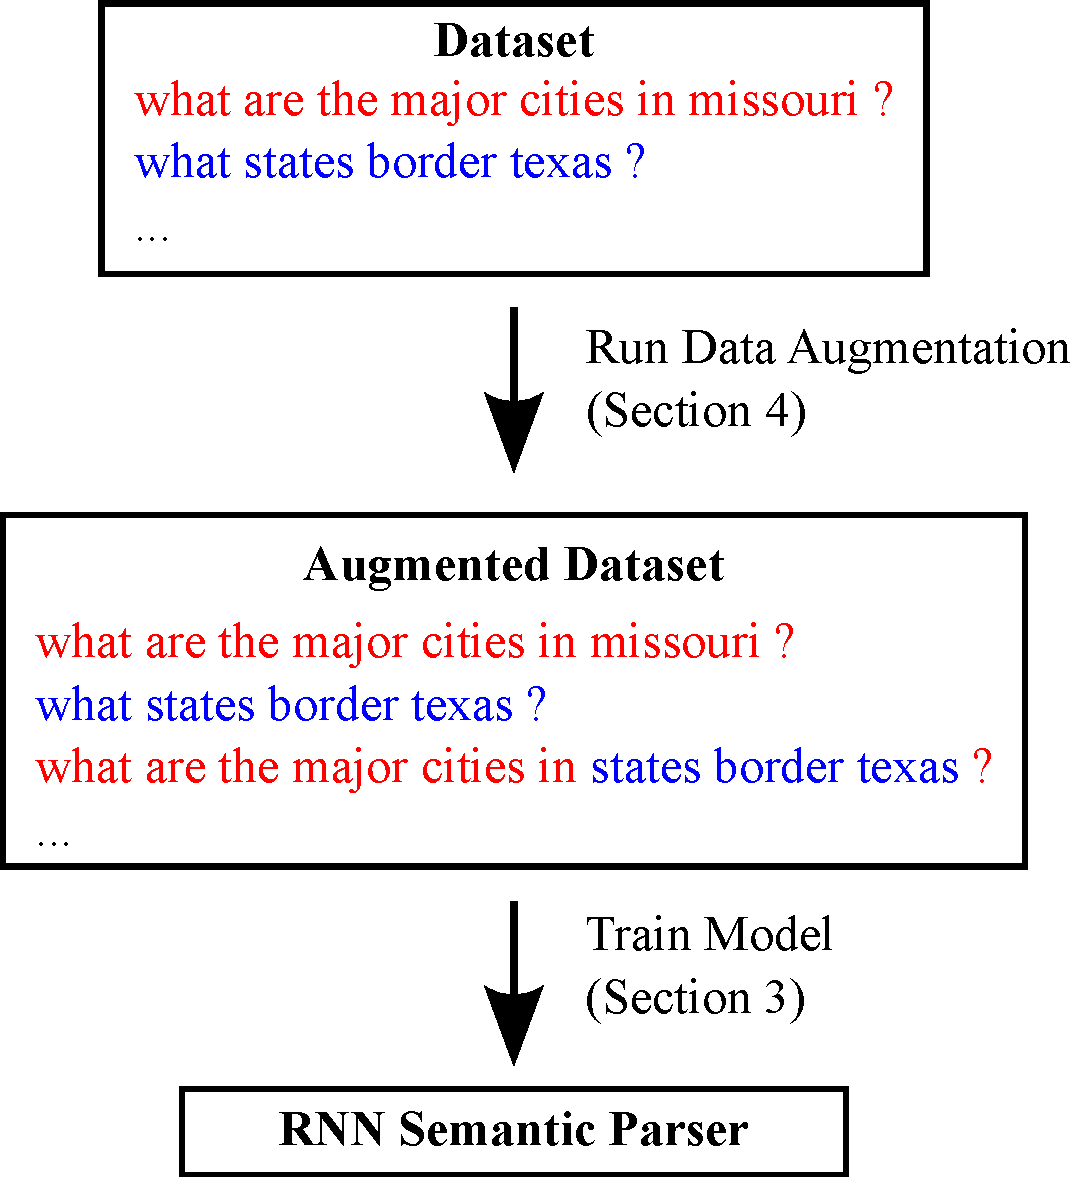
\includegraphics[scale=0.4]{fig-overview.pdf}
\end{center} 
\caption{An overview of our system.}
\label{fig:overview}
\end{figure}

Recently, recurrent neural networks (RNNs) have emerged
as a general-purpose technology for processing sequential data.
In particular, sequence-to-sequence RNN models
have achieved impressive results on a variety of natural language processing
tasks, including machine translation and syntactic parsing.
RNNs are also appealing for their simplicity, as they require 
little hand-engineering of features.

However, there are significant barriers to applying these 
RNN models directly to semantic parsing.
First, semantic parsers are commonly trained from small datasets,
with possibly only hundreds of utterances paired with annotated logical forms.
With this paltry amount of supervision,
RNN models are in danger of severely overfitting the training data.
In particular, RNNs must be able to generalize to a large set of
domain-specific entities which may occur rarely or not at all
in the training dataset.
Second, most modern semantic parsing systems have built-in
prior knowledge about the compositional structure of language.
In contrast, RNNs can only learn about compositionality
through observations of the data.

In this paper, we present the first (to our knowledge)
semantic parser that uses a sequence-to-sequence RNN model to generate
logical forms.  
Our contributions are twofold.
First, we introduce a new RNN sequence-to-sequence model that uses 
attention to handle rare words, such as entity names.
Second, we present a general recipe
for compositional data augmentation that encourages 
the model to learn the compositional structure of language, 
and prevents overfitting.

\cite{liang2013lambdadcs}.

\section{Related Work}
Much excitement currently surrounds sequence-to-sequence RNNs,
which can map input sequences to output sequences.
Such models have been trained on such diverse tasks as
machine translation (CITE), syntactic parsing (CITE), and 
finding convex hulls (CITE), with impressive results on each.
In particular, the recent work on syntactic parsing showed that
RNNs, despite generating output in a linear fashion, can 
learn to generate tree-structured outputs.

Nonetheless, there has yet to be a successful application of
neural networks for semantic parsing.
We are only aware of one previous effort 
(http://yoavartzi.com/sp14/pub/gbfh-sp14-2014.pdf),
though their model was not a sequence-to-sequence model,
and they had yet to achieve good results.

Current semantic parsing systems are
complex and have a great deal of prior knowledge
baked into their internal structure.
One popular approach, CCG, models semantic parsing as 
building a 
Both of these approaches are built to model \emph{compositionality},
the phenomenon that the meaning of an utterance comes from
the meaning of its parts and the way in which they are combined.
To parse an utterance, lexicon rules are applied to
small parts, and then these pieces are combined to form a full
logical form.

Data augmentation has been shown to help neural networks,
particularly in the field of computer vision.
AlexNet, which won COMPETITION, was trained on 
augmented data generated by applying various transformations
to the input images that did not change the label.
In this work, we use a more general form of data augmentation,
in which we simultaneously transform both the input and the output
in a way that preserves the fact that the new output is correct
for the new input.
- AlexNet (http://www.cs.toronto.edu/~fritz/absps/imagenet.pdf) 
- Another nice analysis (http://arxiv.org/pdf/1405.3531.pdf) 

\section{Task}
We model semantic parsing as a generic sequence-to-sequence task.
The input utterance $x$ is tokenized into words $x_1, \dotsc, x_m
\in \vocabin$, the input vocabulary;
similarly, the output logical form $y$ is tokenized
into tokens $y_1, \dotsc, y_n \in \vocabout$, the output vocabulary.

\subsection{Datasets}
\begin{table}[ht]
  \centering
  \small
  \begin{tabular}{|l|c|c|c|}
    \hline
    Dataset & Training Examples & Test Examples \\
    \hline
    \geo & 600 & 280 \\
    \regex & - & - \\
    \hline
  \end{tabular}
  \caption{Overview of the datasets used in this paper.  
  For \geo, we use the standard 600/280 split first used by (CITE).
  For \regex, we create our own split by randomly partitioning
the dataset.}
  \label{tab:datasets}
\end{table}

We present results on a few different standard semantic parsing datasets.

\begin{itemize}
  \item \textbf{ATIS} (\atis).  The ATIS domain contains pairs of
    natural language queries for an airplane flight database
    paired with corresponding database queries written in a 
    lambda calculus-based language.

  \item \textbf{Regular Expressions} (\regex).  The regular expressions domain
contains pairs of natural language descriptions of regular expressions,
paired with associated regular expressions.

  \item \textbf{Geoquery} (\geo).  The geoquery domain
contains pairs of natural language questions about US geography
paired with corresponding database queries written in a prolog-based
query language (CITE).
\end{itemize}

It is notable that these datasets are many orders of magnitude smaller
than the datasets used to train neural machine translation systems (CITE).
Similar work on syntactic parsing achieved good results
when trained on tens of thousands of parse trees.

Our current system does not have the capacity to learn from denotations,
which prevents us from using some other datasets,
such as FREEBASE (CITE).
We explore this more in the Discussion section.

\subsection{Implementation Details}
We tokenize logical forms in a domain-specific manner,
as this depends on the syntax of the formal language being used.
This tokenization is performed in such a way that
entity names can be easily copied from input to output.
At the same time, we intentionally perform name mangling on predicate names,
so that the model cannot cheat with added information.
For example, in the \geo domain, we transform the name
of the predicate ``\texttt{city}'' to ``\texttt{\_city}''
so that the model cannot directly copy the word ``city'' from the input 
to output.

\section{Neural Semantic Parser}
Our neural semantic parser is based closely on existing
attention-based neural machine translation models (CITE).
In particular, we closely follow THANG.

\subsection{Core Model} 
First, we describe the core of our semantic parser,
which is an sequence-to-sequence RNN model with attention.
The system takes as input a sequence $x = x_1 ,\dotsc , x_m$
where each $x_i \in \vocabin$.
Each $x_i$ is mapped to a vector $\phiin(x_i)$.
The encoder module is a bi-directional LSTM, which we define
in more detail below.
The encoder consists of two networks--a forward RNN and backward RNN.
Each RNN starts with a fixed initial hidden state vector $s_0$, and 
generates a sequence of hidden states $h_1, \dotsc, h_m$ by
repeatedly applying the recurrence \[
  h_i = f(u_i, h_{i-1})
\]
for some function $f$,
where $u_i$ is the word vector fed to the network at the $i$-th time step.
For the forward network, this equals $\phiin(x_i)$; for the
reverse network, it is $\phiin(x_{m-i})$.
In this work, we choose $f$ to have the form of an LSTM (CITE).
The word vector function $\phiin$ is shared between the 
forward and backward RNNs, but the internal network parameters are
separate.

Next, we generate annotation vectors $a_i$ for each 
$i \in \{1, \dotsc, n\}$ by concatenating the 
state vector at time $i$ for the forward RNN and time $n-i$ 
for the backward RNN.

Finally, we describe the decoder network.  
Like the encoder, the decoder has a function $\phiout$
that maps words in $\vocabout$ to vectors.
The decoder's initial state $s_0$ is computed from 
the concatenation of the final states of the two encoder RNNs.
In particular, we have \[
  s_0 = W^{(s)} \begin{pmatrix} \overrightarrow{h_m} \\ \overleftarrow{h_m} \end{pmatrix},
\]
for some parameter matrix $W^{(s)}$.
$\overrightarrow{h_i}$ and $\overleftarrow{h_i}$ denote the hidden states
from the $i$-th timestep for the forward and backward encoder RNNs, respectively.

Our decoder uses an attention model similar to that of THANG.
Given the current hidden state $s_j$, our model computes
a context vector $c_j$ as a weighted average of the annotation vectors
computed by the encoder.
At each time $j$, we compute scores for each input word \[
  e_{ij} = s_{j-1}^T W^{(a)} a_i
\]
These are normalized to a probability by a softmax, producing \[
  \alpha_{ij} = \frac{\exp(e_{ij})}{\sum_{i=1}^m \exp(e_{ij})}.
\]
Finally, the context vector is computed as a weighted average of annotations: \[
  c_j = \sum_{i=1}^m \alpha_{ij} a_i.
\]

The decoder generates the $j$-th output word $y_j \in \vocabout$ based on 
the current state $s_{j-1}$ and the annotations $a_1 \dotsc, a_m$;
in the next section, we describe two different output modules.

The state is updated according to the recurrence \[
  s_j = g(v_j, s_{j-1}, c_{j-1}),
\]
where $v_j = \phiout(y_j)$.
The function $g$ is also in the LSTM family.

\subsection{Basic Output Module}
The basic output module uses a simple softmax over all
output vocabulary words, as in other similar works (CITE).
The probability of outputting word $w \in \vocabout$ at time $j$ is \[
  P(y_j = w \mid x, y_{1:j-1}) \propto \exp(U_{w}^T s_{j-1}),
\]
where $U$ is a matrix with rows indexed by elements of $\vocabout$.

\subsection{Attention-based Copying}
One property of semantic parsing tasks is that they have a large
output vocabulary size, compared to the number of training examples.
In particular, semantic parsers must be able to handle a large set of
entity names, which can often be copied directly from the input to the output.
This observation motivates our attention-based copying output module.
We allow the network to copy a word directly from input to output,
with probability determined by the amount of attention paid to that input word.
Mathematically, we let 
\begin{align*}
  P(y_j &= w \mid x, y_{1:j-1}) \propto 
  \\ &\exp(U_{w}^T s_{j-1})
  + \sum_{i=1}^m \mathbb{I}[x_i = w] \exp(e_{ij}),
\end{align*}
where $e_{ij}$ is the attention score described earlier.

We note that our attention-based copying can be seen as a 
combination of a standard softmax output layer
and a pointer network (CITE).  In a pointer network,
the only way to generate output is to copy a symbol from the input,
using an attention mechanism.

\subsection{Learning}
During training, we maximize loglikelihood of the correct
logical form.
This strategy differs from some other semantic parsing systems
(e.g. SEMPRE), which maximize loglikelihood of the correct
denotation.  
We train the model using simple stochastic gradient descent.
Gradients are computed automatically using Theano (CITE).

\section{Data Augmentation}
Semantic parsers are often trained from very small datasets.
Both the \geo and \regex domains have only about $600$ training examples.
By comparison, neural machine translation systems are commonly
trained on datasets with LARGE NUMBER examples.
This small dataset size motivates the development of semantic parsers
that have a lot of built-in knowledge about language.
In particular, standard semantic parsing systems have
the notion of \emph{compositionality} built in.
For example, the Washington SPF (CITE), 
which uses combinatory categorial grammar (CCG),
closely models the alignment between words in the utterance 
and predicates in the logical form, as well as how these parts
combine.  SEMPRE (CITE) similarly builds up logical forms
recursively from smaller sub-units.  In contrast,
our neural semantic parser generates logical forms in a linear fashion,
left-to-right.  It has no prior expectation that language should
exhibit compositionality.

Therefore, we augment our small training datasets with 
more examples generated from a compositional data augmentation scheme.
We perform data augmentation on both \regex and \geo.
In both cases, we cast the problem as one of grammar induction.
We use the existing training examples to induce a
synchronous context-free grammar (SCFG) over utterances and logical forms.
The grammar is designed to be high-precision, 
in that most utterance-logical form pairs generated from the grammar
do in fact match each other.
We then generate new examples from this grammar,
and add these to our original training dataset.
This process is described in more detail for both domains.

\subsection{Augmentation for \regex}
For \regex, our basic strategy is to find small pieces of 
utterances and regular expressions that we can align with high confidence.
We write two rules that capture the primary cases:
\begin{itemize}
  \item Quoted strings.  If a string appears inside quotation marks
    in the utterance, and is found verbatim in the corresponding
    regular expression, we assume that these align directly.
  \item Integers.  If exactly one integer occurs in both the 
    utterance and regular expression, we assume they should be aligned.
    If the integers are not equal, we assume that there should be
    a constant difference between them (see FIGURE for an example).
\end{itemize}

Our grammar therefore has three categories: 
\texttt{\$ROOT}, \texttt{\$QuotedStr}, and \texttt{\$Int}

FIGURE provides more detail about data augmentation on \regex.

\subsection{Augmentation for \geo}
The \geo domain exhibits a greater degree of compositionality
than \regex, which presents an opportunity to use a more sophisticated
data augmentation strategy.
In particular, the more difficult \geo queries tend to have
nested sub-queries (e.g. ``states that border states that border texas'').
% TODO: get a real example

To generate examples with similar nesting structure,
we generate two types of alignments: entity-level and sentence-level.
Entity-level alignments connect mentions of specific states, cities, or rivers
in the utterance to their corresponding mentions in the logical forms.
This can be accomplished with simple string matching.
Sentence-level alignments connect entire utterances to 
corresponding logical forms whose denotations are of a particular 
type (e.g. sets of states, cities, or rivers).
The types are easy to infer based on the logical form alone.

We use both types of alignments to infer grammar rules.
However, when we generate new examples from the grammar,
we do not use the entity-level alignments;
this forces the grammar to generate examples that have 
at least two levels of nesting.

More formally, we have a grammar with four categories:
\texttt{\$ROOT}, \texttt{\$State}, \texttt{\$City}, and \texttt{\$River}.
We chose the last three because they are the most common entity types
that appear in the dataset.  

FIGURE provides more detail about data augmentation on \geo.

\section{Experiments}
We evaluate our system on three domains: \atis, \regex, and \geo.
For the \atis domain, we report exact logical form match accuracy.
For \regex, we determine correctness of a predicted regular expression
by first converting it and the gold regular expression to
deterministic finite automata (DFAs).  We then call the regular expressions
equivalent if and only if corresponding automata are equivalent.
This procedure is guaranteed to call two regular expressions equivalent
if and only if they define the same regular language (CITE).
Finally, for \geo, we determine correctness based on denotation match.

We compare our full system described in section (LINK), \textbf{\attncopy}, 
to two related baselines:
\begin{itemize}
  \item \textbf{\encdec}.  An encoder-decoder LSTM model with no copying module.
  \item \textbf{\attn}.  The LSTM model with attention described in section (LINK),
     but with no copying module.
\end{itemize}

Name mangling and copying when comparing to Liang 2011

\subsection{Implementation Details}
We ran all experiments with a hidden size of $400$ units,
and $50$-dimensional word embeddings.
We initialized all parameters uniformly at random 
within the interval $[-0.1, 0.1]$.
We used a simple learning rate schedule:
we first train the model for $25$ epochs at a learning rate of $0.1$,
then for $5$ more epochs with a learning rate of $0.05$,
and finally $5$ additional epochs with a learning rate of $0.025$.
For the \attncopy model, we replace word vectors for words
that occur only once in the training set 
with a universal \texttt{<unk>} word vector;
we do not do this for the baselines, as without the copying mechanism,
replacing rare words with \texttt{<unk>} hurts performance.

Another important hyperparameter for \regex and \geo is the
extent to which we perform data augmentation.
For \regex, we train on the original dataset,
plus all NUMBER examples generated by the integer-based scheme
and $1000$ randomly sampled new examples generated by the string-based scheme.
For \geo, we train on the original dataset,
plus $2000$ randomly sampled new examples.
All hyperparameters were tuned by training on a subset of the
training set, and evaluating on the remaining examples.

At test time, we use beam search with beam size $K=10$.
We automatically balance missing right parentheses.
We then pick the highest-scoring parse 
that can be processed by our domain-specific
equivalence-checking routine without errors.
On \geo, this means we take the highest-scoring parse
that does not yield an executor error when the
corresponding denotation is computed;
on \regex, this means that no error is thrown when 
converting the regular expression to a DFA.

\subsection{Main Results}
First, we evaluate our system trained on the original dataset alone,
and no new examples generated by our data augmentation approach.
Our results are summarized in the second group of rows of Table \ref{tab:results}.
Note that even without data augmentation, we are able to nearly
match the state-of-art on the \regex dataset.
However, we lag significantly behind on \geo.

Next, we now rerun our system and all baselines on our
augmented training datasets.  These results are shown in the
third and final group of rows of Table \ref{tab:results}.
With data augmentation, we achieve a new state-of-art level performance
on \regex, by a considerable margin.  We are also much more competitive
with state-of-art on \geo.

\begin{table}
  \centering
  \small
  \begin{tabular}{|l|c|c|c|}
    \hline
    System & \atis & \regex & \geo \\
    \hline
    Zettlemoyer 2007 & $84\%$ & & \\
    Kushman 2013 & & $67\%$ & \\
    Liang 2011 & & & $91\%$ \\
    \hline
    \textbf{Original Dataset} & & & \\
    \encdec & - & - & - \\
    \attn & - & - & - \\
    \attncopy & $78.3$ & $65.0$ & $75.0$ \\
    \hline
    \textbf{With Data Augmentation} & & & \\
    \encdec & & - & - \\
    \attn & & - & - \\
    \attncopy & & $79.0$ & $84.0$ \\
    \hline
  \end{tabular}
  \caption{Results.}
  \label{tab:results}
\end{table}


\subsection{Learning Compositionality via Alignments}
TODO: look at attention weights

We know that the attention-based copying results in
better attention alignments.
Adding the augmented data makes this even better.

\subsection{Real vs. Augmented Data}
We ran additional experiments on \geo to characterize
the extent to which data augmentation helps our system.
In particular, we wanted to compare the increase in performance
caused by adding synthetic data to the 
increase in performance caused by adding more actual examples.

In Figure FIG, we plot dev accuracy as a function of
the number of real training examples.  The red line
shows results without data augmentation;
the blue line shows results when data augmentation was 
performed on the available training examples.
From this plot, we see that the effect of 
data augmentation is relatively constant regardless
of original training set size; if anything,
it helps slightly more when there is more training data.
On the other hand, there are clear diminishing marginal returns
to adding real training examples, and the curve appears to level out
significantly below the curve for augmented data,
suggesting that the compositionally-generated data
provides a significant boost that could not be replicated
by annotating a few more examples.

\subsection{Data Augmentation and Covariate Shift}
We have shown that data augmentation can yield significant improvements
for our model, as it encourages the model to learn good alignments,
a simple form of compositionality.  Nonetheless,
there are also drawbacks to our data augmentation, as it introduces
covariate shift: certain types of examples are more likely than others
to occur in our augmented data.

To illustrate the effects of covariate shift, we ran an additional
experiment on the \regex dataset.  We trained our model
on the original dataset plus augmented data generated only from the
integer-based scheme; we also trained a separate copy of the model
on the original dataset plus augmented data generated only from the
string-based scheme.  

The results of this experiment are summarized in Table \ref{tab:regex-shift}.
We see that in isolation, each individual data augmentation scheme
does not significantly help accuracy.
The integer-based augmentation helps the model deal better
with utterances that contain an integer 
(third column of Table \ref{tab:regex-shift}),
but hurts performance on other examples.
Similarly, the string-based augmentation helps the model
deal better with utterances that contain quoted strings 
(fourth column of Table \ref{tab:regex-shift}),
but hurts performance on other examples.
Pooling both sources of augmented data improves performance
across the board.

\begin{table*}
  \centering
  \small
  \begin{tabular}{|l|c|c|c|}
    \hline
    Dataset & Accuracy & Accuracy on Int Examples & Accuracy on String Examples \\
    \hline
    Original & $65.0$ & $11/19$ & $54/82$ \\
    Int-Augmented & $67.0$ & $15/19$ & $52/82$ \\
    String-Augmented & $65.0$ & $8/19$ & $56/82$\\
    All Augmented & $79.0$ & $17/19$ & $62/82$ \\
    \hline
  \end{tabular}
  \caption{Results.}
  \label{tab:regex-shift}
\end{table*}

\section{Discussion}
In this paper, we have presented the first RNN sequence-to-seqeunce
model for semantic parsing.  Our model is easy to train
and gives good performance on a wide variety of semantic parsing
datasets, when trained with logical form supervision.
Additionally, we describe a data augmentation approach that 
further boosts performance by (REASONS).

While our data augmentation techniques have been effective,
they did require some manual processing.
One line of potential future work would be to
perform automatic grammar induction.
We could leverage existing work on semantic parsing
using semantic unification (CITE).

One limitation of our approach is that it must learn from annotated logical forms.
In the last few years, there has been an emergence of
semantic parsers that can learn from denotations (CITE).
Such systems have a built-in understanding of the space of
syntactically valid logical forms, which our RNN semantic parser lacks.
Similarly to our data augmentation, we could try to
teach the parser this information by using synthetic data.
For example, we could initialize the system 
by generating canonical utterances for logical forms,
as in (OVERNIGHT).  We would first train the system to map
canonical utterances to logical forms, so that it would learn to produce
valid logical forms that are related to the input;
then, we would add in more data that pairs real utterances with denotations.

An alternative direction would be to incorporate the execution
step altogether.  Recent work on the Neural Enquirer (CITE)
explores the idea of having a neural network learn to map
SQL queries to denotations.  Such a system could be trained
on natural language queries instead of SQL.
Another piece of work in this vein is (WESTON SIMPLE QUESTIONS);
they too replace a database query engine with a neural network
whose ``memories'' encode all the relations in the database.

\section*{Acknowledgments}
Do not number the acknowledgment section.

\section*{Reproducibility}
All experiments will be available on 
\url{http://www.codalab.org}

\bibliography{all}
\bibliographystyle{naaclhlt2016}


\end{document}
